\documentclass[10pt,twocolumn]{article}
\usepackage[letterpaper,margin=1.8cm,headheight=15pt,headsep=18pt]{geometry}
\usepackage[T1]{fontenc}
\usepackage{lmodern,amsmath,amssymb,graphicx,booktabs,xcolor,tikz,fancyhdr}
\usepackage[colorlinks=true,linkcolor=teal,citecolor=teal,urlcolor=teal,pdfauthor={Pipit},pdftitle={The Coherence Atlas: A Tutorial Paper}]{hyperref}
\definecolor{pine}{HTML}{234D3D}
\definecolor{gold}{HTML}{A36B22}
\definecolor{mist}{HTML}{EDF3EB}
\pagestyle{fancy}\fancyhf{}\fancyhead[L]{\small\textsc{Pipit / The Coherence Atlas}}\fancyhead[R]{\small Tutorial paper}
\fancyfoot[L]{\scriptsize Instructional specimen. All observations are synthetic.}\fancyfoot[R]{\small\thepage}
\setlength{\columnsep}{24pt}
\setlength{\parskip}{5pt}
\setlength{\parindent}{0pt}
\newcommand{\key}[1]{\texttt{#1}}
\newcommand{\mission}[2]{\par\medskip\noindent\fcolorbox{pine}{mist}{\parbox{\dimexpr\columnwidth-2\fboxsep-2\fboxrule}{\small\color{pine}\textbf{#1}\\#2}}\par\medskip}
\newcommand{\tagline}[1]{{\small\color{gold}\textsc{#1}}\par\medskip}
\begin{document}
\twocolumn[{
\begin{center}
{\small\color{pine}\textsc{An interactive field guide / Pipit Tutor}}\par\vspace{12pt}
{\LARGE\bfseries The Coherence Atlas}\\[5pt]
{\Large A Tutorial Paper for Reading Connected Evidence}\\[10pt]
{\normalsize Pipit Learning Lab}\\[3pt]
{\small A fictional research specimen, designed for hands-on practice}\\[12pt]
\end{center}
\begin{abstract}
Research reading combines local inspection with deliberate navigation: finding a term, checking an equation, comparing passages, and preserving useful evidence. This tutorial models those actions as a small exploration of coherence in synthetic signals. The paper contains real PDF text, numbered equations, linked citations, a figure and a table. Its scientific observations are invented teaching data, not experimental findings. Run \texttt{:Tutor} in Pipit to turn this paper into guided missions with local progress, points and optional challenges. No account or online citation lookup is needed to complete the tutorial.
\end{abstract}\vspace{14pt}
}]
\section{An invitation to investigate}
A useful result is rarely understood in isolation. Its symbols must be defined, its evidence inspected, and its sources considered. Our specimen asks a simple question: when do repeated observations tell a coherent story?
The word \emph{coherence} is the first search target. Later pages introduce a scoring rule and a synthetic experiment. Your task is not to memorize them, but to learn how to move between them without losing your reading position.
\mission{Start the expedition}{Open Pipit's command menu with \key{:}, type \key{Tutor}, and press Enter. The on-screen tutor checks real reader actions; the paper itself remains an ordinary PDF.}
\subsection{Your route}
Page 2 introduces the navigation task. Page 3 defines the model, including \hyperref[eq:coherence]{equation (2)}. Page 4 supplies a figure and a table. Page 5 offers comparison and note-taking challenges. Page 6 contains references and a final checklist.
\section{How to read this specimen}
Follow the mission panel at your own pace. Use either the mouse or the keyboard. The same action can be found through the command menu if a shortcut conflicts with your browser.
The reference lens is a temporary window into a different part of this PDF. It can be pinned for side-by-side reading. In a two-column paper, its initial view follows a detected column rather than shrinking an entire page.
\mission{A reference to try}{Preview \hyperref[eq:coherence]{equation (2)}, then inspect \hyperref[tab:results]{Table 1} and \hyperref[fig:signals]{Figure 1}. A wrong crop is recoverable: use \key{g P} for the full page.}
\subsection{A fair learning loop}
The tutor awards points for completed actions, not for waiting. There are no streak penalties, countdowns, purchases or leaderboards. Hints are free. Skipping a mission does not award its points and does not block later practice.
This structure follows the practical idea that tools should help us revisit evidence rather than merely display it \cite{bush}. The score is a record of practice, not a scientific reading assessment.
\newpage
\tagline{Waypoint 1 / Learn the terrain}
\section{Methods: locating evidence}
A page number is a coordinate, not a complete reading position. Useful navigation preserves both the page and its scroll position. Pipit records a reading trail when you follow references and make jumps.
\subsection{A navigational protocol}
Start with the page command: press \key{p}, enter a page number, and confirm. The outline is available with \key{t}. A mouse user can choose the page control or contents from the dock.
\mission{Mission: reach this page}{Navigate from page 1 to page 2. Use the page command, the dock, the outline, or scrolling. The tutor notices the actual page change.}
\subsection{Search before scanning}
Find \emph{coherence} with \key{/}. The search reads the PDF's text layer and highlights matches. Move between matches with \key{n} and \key{N}. This is ordinary searchable text, not a picture of a page.
Search can fail on scans or unusual encodings. A zero-result search is not evidence that a concept is absent from the underlying scanned document.
\mission{Mission: find the signal}{Search for \key{coherence}. A visible search result completes the mission. Close the search bar with Escape when you are ready to inspect a reference.}
\subsection{Return points}
After jumping from this page to a definition, \key{Alt+Left} returns through the reading trail. \key{Alt+Right} moves forward. The arrow keys alone still serve ordinary navigation contexts.
\section{What the experiment is not}
The numerical values in this paper are fabricated, consistent teaching examples. They do not establish an improvement over another PDF reader or a theory of human learning.
Our only testable interface claim is local: if the reader exposes an action and the tutor observes its successful outcome, that mission can be marked complete.
\subsection{Bookmarks and marks}
Bookmarks persist locally. Press \key{b} to toggle one at the current page and \key{Shift+B} to inspect your list. Named marks use \key{m} followed by a letter; an apostrophe followed by the letter returns to that mark.
\mission{A useful habit}{Bookmark a page before exploring its references. The point is to preserve a route back, not to collect bookmarks for their own sake.}
\subsection{A note on source connections}
The bibliography on page 6 is small and fully local. Citations link to actual entries inside this PDF. Broader citation maps are a separate, optional network feature and are not needed for the tutor.
\subsection{A hidden landmark}
The phrase \emph{the atlas remembers} appears here as an optional search landmark. Find it when you want to practice a more specific query after finishing the main search mission.
\newpage
\tagline{Waypoint 2 / Inspect the model}
\section{A model of coherent evidence}
Let $x_i$ denote a synthetic observation and $w_i$ its non-negative weight. We normalize the weights so that $\sum_i w_i=1$. A weighted mean summarizes the observations:
\begin{equation}
\mu=\sum_{i=1}^{n} w_i x_i .
\label{eq:mean}
\end{equation}
A toy coherence score penalizes dispersion around that mean:
\begin{equation}
C=\frac{1}{1+\sum_{i=1}^{n}w_i(x_i-\mu)^2}.
\label{eq:coherence}
\end{equation}
Here $0<C\leq1$ for finite observations. This is only a teaching definition, not a validated metric for research quality.
\mission{Mission: inspect equation (2)}{Press \key{e}, type \key{2}, and press Enter to preview the equation. Alternatively, use \key{F} over a visible reference and type its hint. The tutor waits for a rendered preview.}
\subsection{Why definitions matter}
The denominator in equation (2) combines normalization and variance. An interpretation that ignores either term would overstate what the score measures. The quantity is deliberately simple enough to compare against \hyperref[tab:results]{Table 1}.
\subsection{The lens as a working surface}
Scroll inside a preview to reveal more context. Use \key{Alt+PageUp} and \key{Alt+PageDown} to navigate its pages independently. The main document stays in place.
\section{Comparing a claim with its definition}
A pinned lens is useful when a later paragraph depends on a symbol introduced several pages earlier. Keep equation (2) visible while reading the synthetic results.
\mission{Mission: pin a reference}{With the preview open, press \key{Shift+P} or use its context menu to pin it. Resize the divider with the mouse, or focus it and use the arrow keys.}
\subsection{A derived comparison}
If all observations are identical, then $C=1$. If the weighted dispersion is $v$, then
\begin{equation}
C(v+\Delta v)-C(v)
=-\frac{\Delta v}{(1+v)(1+v+\Delta v)} .
\label{eq:change}
\end{equation}
For a positive change in dispersion, the score decreases. This is an algebraic property of our definition, not a statement about a physical system.
\subsection{Read both columns}
This page deliberately uses two columns. Previewing a definition should initially fit its column. A full-width figure may need different bounds; use the full-page fallback whenever an automatic crop omits relevant content.
\mission{Mission: follow and return}{Choose Follow passage from the preview's context menu (or focus the preview and press Enter), then use \key{Alt+Left} to return. The tutor checks that a real history return occurred.}
\newpage
\tagline{Waypoint 3 / Check a figure and table}
\section{Synthetic observations}
Figure 1 shows two invented traces. Their colors provide a useful test of reading palettes: a theme should preserve distinguishable lines, but only original colors should be trusted for color-critical interpretation.
\begin{figure}[h]
\centering
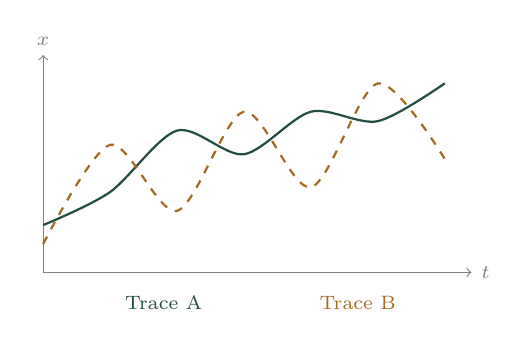
\begin{tikzpicture}[x=.85cm,y=.60cm]
\draw[->,gray] (0,0)--(6.4,0) node[right,font=\scriptsize] {$t$};
\draw[->,gray] (0,0)--(0,4.6) node[above,font=\scriptsize] {$x$};
\draw[pine,thick] plot[smooth] coordinates {(0,1)(1,1.7)(2,3)(3,2.5)(4,3.4)(5,3.2)(6,4)};
\draw[gold,thick,dashed] plot[smooth] coordinates {(0,.6)(1,2.7)(2,1.3)(3,3.4)(4,1.8)(5,4)(6,2.4)};
\node[pine,font=\scriptsize] at (1.8,-.65) {Trace A};
\node[gold,font=\scriptsize] at (4.7,-.65) {Trace B};
\end{tikzpicture}
\caption{Synthetic traces, drawn as vector graphics. Solid and dashed styles distinguish them independently of color.}
\label{fig:signals}
\end{figure}
\subsection{Tabulated dispersion}
\begin{table}[h]
\centering
\begin{tabular}{lrr}
\toprule
Condition & Dispersion $v$ & $C(v)$\\
\midrule
Aligned & 0.10 & 0.909\\
Mixed & 0.40 & 0.714\\
Dispersed & 1.00 & 0.500\\
\bottomrule
\end{tabular}
\caption{Invented values consistent with equation (2), rounded to three decimals.}
\label{tab:results}
\end{table}
\mission{Optional inspection}{Look up \key{figure 1} or \key{table 1} with the figure/table command \key{v}. Compare a content preview with the complete page.}
\section{Appearance is a reading tool}
A bright paper background may suit daylight; a low-luminance palette may suit a dim room. Neither changes the logic of a result. Theme changes do alter the displayed colors of figures.
\mission{Mission: change a theme}{Use \key{g d} to cycle themes, or choose a named theme in the command menu. You can return to your preferred theme afterward.}
\subsection{Reversible choices}
Use \key{g r} to toggle recoloring. Custom foreground and background values are available in settings. For a scientific plot whose exact colors matter, restore original colors before drawing conclusions.
\subsection{Margins and geometry}
Smart width (\key{W}) fits detected text bounds, excluding outer margins. Facing pages (\key{g 2}) provide another view of the same document. These are interface choices, not changes to the PDF file.
\subsection{One question to keep}
Which operation would best test a claim: making its graph more attractive, or checking its definition and numerical assumptions? A notebook entry can preserve your answer with the source page.
\newpage
\tagline{Waypoint 4 / Preserve the evidence}
\section{A reading notebook}
Good notes identify both a passage and why it matters. They can record a question, a disagreement, or the assumption that makes a result applicable.
\mission{Mission: save a note}{Select a passage and press \key{q} to capture it, or open the notebook with \key{Shift+Q} and add a text note. Enter a useful sentence; the tutor checks saved note content rather than merely opening the panel.}
\subsection{Anchors and portability}
Pipit keeps notes separately from the original PDF. A notebook backup is a JSON sidecar; Markdown export includes readable quotes and page references. These exports are not PDF-embedded annotations.
Do not mistake browser storage for a permanent archive. Export important notes before switching profiles, reinstalling extensions, or clearing local data.
\subsection{The specimen's key passage}
\begin{quote}
A reference is useful when it preserves enough context to let a reader check the claim, not merely repeat it.
\end{quote}
This sentence is a convenient target for quote capture. You may instead write your own note about equation (2), Figure 1, or the synthetic values in Table 1.
\mission{Mission: leave a bookmark}{Toggle a bookmark for this page. If it is already bookmarked, remove it and add it again to practice the action.}
\section{Optional challenges}
The main route teaches essential actions. Two optional challenges introduce layout and focus aids. You may skip either without losing completed progress.
\mission{Bonus: read with a ruler}{Enable the reading ruler with \key{r}. Move it with the bracket keys. Disable it when it no longer helps.}
\mission{Bonus: compare facing pages}{Toggle two-page view with \key{g 2}. Notice that layout changes do not alter the document's text or page numbering.}
\subsection{A final comparison}
Return to the mean in equation (1), then the dispersion penalty in equation (2). Explain their relationship in one sentence. This is a self-check, not an automatically graded examination.
\subsection{What your score means}
Points record which reader actions you practiced. They do not measure intelligence, attention, learning speed or scientific understanding. There is no time limit and no reward for keeping the application open.
\newpage
\tagline{Waypoint 5 / A reusable reading route}
\section{Discussion and checklist}
A small set of reversible actions can support careful reading: locate, inspect, compare, return, record. You can now apply that route to your own papers.
\begin{enumerate}
\item Find a specific term in the text layer.
\item Preview a numbered definition without losing your paragraph.
\item Pin context for comparison.
\item Follow a reference and use history to return.
\item Preserve a page-linked note and a bookmark.
\end{enumerate}
\subsection{Take the tools, not the score}
Open your own PDF when you are ready. Leaving the tutor pauses it. Your progress stays on this device, and \key{:Tutor} can resume the route later.
\subsection{Further reading}
The sources below are real publications, included as navigational examples rather than evidence for the invented observations. Citations in this paper use linked numeric markers.
\begin{thebibliography}{9}
\bibitem{bush} V. Bush. As We May Think. \emph{The Atlantic}, 1945.
\bibitem{shannon} C. E. Shannon. A Mathematical Theory of Communication. \emph{Bell System Technical Journal}, 27, 379--423 and 623--656, 1948.
\bibitem{tufte} E. R. Tufte. \emph{The Visual Display of Quantitative Information}. Graphics Press, 1983.
\end{thebibliography}
\section{Reference practice}
The distinction between a source and a claim is central to reading. Bush's essay \cite{bush} offers historical context for linked information. Shannon's paper \cite{shannon} supplies an example of a precisely defined quantity. Tufte's book \cite{tufte} offers a source for thinking about visual explanation.
No network lookup is needed to preview these bibliography entries. The local reference graph can show numeric citation mentions inside this PDF.
\mission{Your next paper}{Close the tutor panel whenever you choose. Open a local PDF with \key{o}, or use the URL command \key{g o}. The commands you practiced remain available outside the tutorial.}
\subsection{Accessibility and pace}
All tutorial controls can be reached with Tab and activated with Enter or Space. Hints are free, progress is local, animations respect reduced-motion settings, and no mission requires online access.
\end{document}
